%%%%%%%%%%%%%%%%%%%%%%%%%%%%%%%%%%%%%%%%%%%%%%%%%%%%%%%%%%%%%%%%%%%%%%%%%%%%
% AGUJournalTemplate.tex: this template file is for articles formatted with LaTeX
%
% This file includes commands and instructions
% given in the order necessary to produce a final output that will
% satisfy AGU requirements, including customized APA reference formatting.
%
% You may copy this file and give it your
% article name, and enter your text.
%
%
% Step 1: Set the \documentclass
%
%

%% To submit your paper:
\documentclass[draft]{agujournal2019}
\usepackage{url} %this package should fix any errors with URLs in refs.
\usepackage{lineno}
\usepackage[inline]{trackchanges} %for better track changes. finalnew option will compile document with changes incorporated.
\usepackage{soul}
\usepackage{caption}

\linenumbers

\draftfalse



\journalname{Geophysical Review Letters}


\newcommand{\markred}[1]{\textcolor{red}{#1}}
%\newcommand{\markcyan}[1]{\textcolor{cyan}{#1}}
\newcommand{\markblue}[1]{\textcolor{blue}{#1}}
%\newcommand{\markgreen}[1]{\textcolor{magenta}{#1}}


\begin{document}



\title{Local hydraulic resistance in heterogeneous porous media}


\authors{Quirine Krol \affil{1}, Itzhak Fouxon \affil{1,2}, Pascal Corso \affil{1}, Markus Holzner \affil{1,2,3,4}}



\affiliation{1}{ETH Zurich, Stefano Franscini-Platz 5, 8093 Zurich, Switzerland}
\affiliation{2}{Department of Computational Science and Engineering, Yonsei University, Seoul 120-749, South Korea}
\affiliation{3}{Swiss Federal Institute for Water Science and Technology EAWAG}
\affiliation{4}{Swiss Federal Institute for Forest, Snow and Landscape Research WSL}



\correspondingauthor{Quirine Krol}{quirine.krol@protonmail.com}



\begin{keypoints}
\item We introduce a new definition for individual pores in heterogeneous porous media based on iso-pressure surfaces.
\item We employ direct numerical simulations to measure the local hydraulic conductivity and revisit the classical model of pore resistance based on Hagen-Poiseuille law. 
\item We model the local hydraulic resistance of a pore based on local circularity and channelization of iso-pressure surfaces. While Hagen-Poisseuille may locally be off with mean relative error of $40\%$, our new model based reduces it to $22\%$ .
\end{keypoints}


\begin{abstract}
[ Resolving local velocities for laminar flow in porous media is essential to transport processes. Using direct numerical simulations to solve the Navier-Stokes equations is computationally costly for statistical representative volumes. Pore network models allow for much faster solutions and resolve much larger domains. However, the pore network architecture and constitutive model for the hydraulic resistance heavily influence the permeability and the quality of local velocity predictions. Here, we investigate the validity of a commonly used constitutive law. We start by generating three three-dimensional artificial geometries with porosities given by $0.68, 0.34, \rm{and } 0.17$ with thresholding Gaussian random fields. As a benchmark, we use high fidelity numerical simulations of the Navier-Stokes equations to resolve the pressure and velocity field for laminar flow in the pore-space of the artificial geometries. We propose a new definition for pores based on iso-pressure surfaces and topology changes that enables us to measure the local hydraulic resistance. We show that the Hagen-Poisueille (HP) model overestimates the local hydraulic resistance up to one order of magnitude. We propose a new constitutive model that is based on the geometry of iso-pressure surfaces. This model shows that the circularity of iso-pressure surfaces is key to predict the local hydraulic resistances of pores in heterogeneous porous media. This model improves the root-mean-squared-relative error from $59\%, 37\%, 24\%$ for the HP model to $20\%, 25\%, 21\%$ for the three porous media respectively. We anticipate that our approach may find broad application in pore network models.]
\end{abstract}

\section*{Plain Language Summary}
[ enter your Plain Language Summary here or delete this section]


%% ------------------------------------------------------------------------ %%
%
%  TEXT
%
%% ------------------------------------------------------------------------ %%

%%% Suggested section heads:
\section{Introduction}

Porous media flow is important for a wide range of applications in nature and technology, spanning from groundwater remediation and oil recovery to packed bed reactors and particle filters. In these flows, the highly complex and three-dimensional pore geometries give rise to complicated pore velocity fields that form the backbone for transport, mixing and chemical reaction processes. Detailed knowledge of these velocity fields is important for the modelling of effective parameters, most notably the permeability and the prediction of transport in porous media \cite{bear_dynamics_1972,scheidegger_physics_1974}. Despite its importance and extensive research, however, the relation between geometrical features of porous media and the resulting flow is still not fully understood.


Given that detailed knowledge of geometrical features of porous media is often unavailable, the classical flow modeling approach has been to represent the porous medium as a lattice of circular tubes that represent the pore network \cite{scheidegger_physics_1974}. The flow in the tubes is assumed uniform and the velocity profile parabolic. While this is a rather crude approximation of the real geometry and flow behaviors, it has provided useful predictions for flow and transport. Early studies have modelled velocity distributions \cite{haring_statistical_1970}, permeability \cite{fatt_network_1956,katz_quantitative_1986} and particle dispersion \cite{saffman_theory_1959} based on bulk statistics of the medium geometry such as pore size distributions. These early studies have spurred many subsequent works on statistical pore scale models e.g. \citeA{dullien_single_1975,kutsovsky_nmr_1996,maier_simulation_1999,de_anna_prediction_2017} and \citeA{dentz_mechanisms_2018}. The second class of models that hinges on the simplified lattice representation of porous media are the so-called pore network models \cite{thompson_modeling_1997}. For both classes of models, the simplified modelling of local hydraulic resistance of individual pores based on Hagen-Poiseuille is a central element.


Many authors tried to relate the statistics of pore velocity to statistics of pore geometry represented by e.g. the local pore radius, the connectivity between pores etc. For example, one of the simplest models is the so-called \emph{capillary bundle} model, in which the porous medium is conceptualized as a parallel arrangement of capillaries with given pore sizes \citeA{scheidegger_physics_1974}. Extensions of this model include parallel arrangements of wavy tubes \citeA{le_borgne_effective_2011}. These simple models are not appropriate for complex porous media, for which the network aspect is important. That is, in general, the connectivity between pores cannot be neglected and the concept of the linear pore breaks down \citeA{dentz_mechanisms_2018}. An ad-hoc model that conceptualizes flow in porous media as a system of serial and parallel pore arrangements can be found in \cite{holzner_intermittent_2015}. \cite{siena_relationship_2014} and \cite{hyman_heterogeneities_2012} statistically related velocity distributions to pore size distributions of statistically generated 3D porous media. Based on direct numerical simulations in 2D porous media composed of disks, \cite{de_anna_prediction_2017} showed that the low velocity tail of the pore velocity distribution is governed by local pore size. This is a notable result as it suggests that the slow flow velocities are not strongly dependent on the connectivity between pores. \cite{alim_local_2017} showed that pore velocity distributions are governed by local correlations of pore sizes that organize flux ratios at pore junctions, while pore size itself was a poor predictor of flux ratios. They simplified two-dimensional porous medium flow by a network of tubes with varying diameter and the flow within each tube was calculated by solving for Kirchoff’s circuit law for two-dimensional Poiseuille flow within the tubes of rectangular cross section. Even though using tubes with varying diameter is a refinement compared to simpler models with tubes of constant diameter, the simplification with respect to real geometries is still strong. Despite this, a comparison of simulation results with the experimentally obtained velocity distribution in a two-dimensional micromodel composed of pillars showed reasonable agreement \citeA{alim_local_2017}. As mentioned, the statistical models in these works are based on the concept that local velocity profiles are parabolic. Some recent papers provided qualitative examples comparing pore velocity profiles to a parabola that suggest the assumption may be reasonable \citeA{de_anna_prediction_2017,dentz_mechanisms_2018} and some evidence is provided by the comparison between simulations and experiments by \cite{alim_local_2017}. However, a rigorous assessment of local hydraulic resistance in three-dimensional pore geometries is still missing in the literature. 


With the advent of experimental techniques like micro-computed tomography there is now access to impressive details of three dimensional porous media architectures. Even though today’s computing facilities make it possible to solve flow and transport with unprecedented accuracy in these complex geometries using direct numerical simulations, this approach is only feasible in small domains. Simple models that reduce the full complexity of real porous media are still needed. A lattice representation is the standard approach in so-called pore network models in which a Kirchhoff-type system of equations is solved to model single or multiphase porous medium flows \citeA{thompson_modeling_1997}. The lattice is usually constructed based on data from experimental pore scale characterization measurements, e.g. imaging or mercury intrusion porosimetry. These pore network models are a valuable tool for understanding meso-scale phenomena, linking single pore processes and continuum porous media used in engineering \citeA{xiong_review_2016}. Besides a sound network construction approach that mimics the real media, another critical aspect for the accuracy of modeling is the representation of local hydraulic resistance in the pores. 


In this paper we start with a theoretical background where we define local pores based on consecutive iso-pressure surfaces, followed by a new model for the local hydraulic conductivity. In the methods section we describe our numerical experiment consisting of direct numerical simulations (DNS) from which we obtain local velocity and pressure data in heterogeneous porous media. Based on a post-processing of the DNS data we can extract the local hydraulic conductivity of a local pore. In the results we compare the measured hydraulic resistances to the Hagen-Poiseuille model and to the newly formulated model based a local shape parameter circularity. In the discussion we treat the limitations and extrapolations of the newly proposed model. In the conclusion we state the model performance compared to the HP model.



\section{Theoretical Background}

For low Reynolds numbers and incompressible flow, the local flow in a porous media is described by the Stokes equations,
\begin{equation}
	\mathbf{\nabla} p =  \mu\mathbf{\nabla}^2 \mathbf{u}\,,~~~\mathbf{\nabla}\cdot\mathbf{u}=0\label{eq:stokes_local}
	\end{equation}
with pressure $p$ and velocity $\mathbf{u}$ and dynamic viscosity $\mu$. For an arbitrary volume $\mathcal{V}$ in a porous media, enclosed by surface $\partial \mathcal{V}$ given by two iso-pressure surfaces $S_{p_1}$ and $S_{p_2}$ and a remaining a porous media domain $\Gamma$, we can write down the integral form of the Navier-Stokes equations
{}

\begin{equation}
\int_{\mathcal{V}} \left(\mathbf{u}\cdot\mathbf{\nabla} p-\mu \mathbf{u}\cdot\mathbf{\nabla}^2 \mathbf{u}\right) dV 
= \int_{\partial \mathcal{V}}  p\,\mathbf{u}\cdot\mathbf{n}\,dS+\mu \int_{\partial \mathcal{V}} \mathbf{u} (\mathbf{\nabla} \mathbf{u})\cdot\mathbf{n}\,dS-\mu \int_{\mathcal{V}} (\mathbf{\nabla}\, \mathbf{u})^2 dV=0. \label{eq:stokes_dissipation}
\end{equation}

Given that at the porous media boundary domain $\Gamma$ we have a no-slip condition $\mathbf{u}=0$ we can write 
\begin{equation}
	Q \Delta p = -\mu\int_{S_{p_1}+S_{p_2}} \mathbf{u} (\mathbf{\nabla} \mathbf{u})\cdot\mathbf{n}\,dS +\mu \int_V (\mathbf{\nabla}\, \mathbf{u})^2 dV, \label{eq:pressuredrop}
\end{equation}
with the total flux defined by 

\begin{equation}
	Q=\int \mathbf{u}\cdot\mathbf{n}\, dS.
\end{equation}


\begin{figure}[t!]
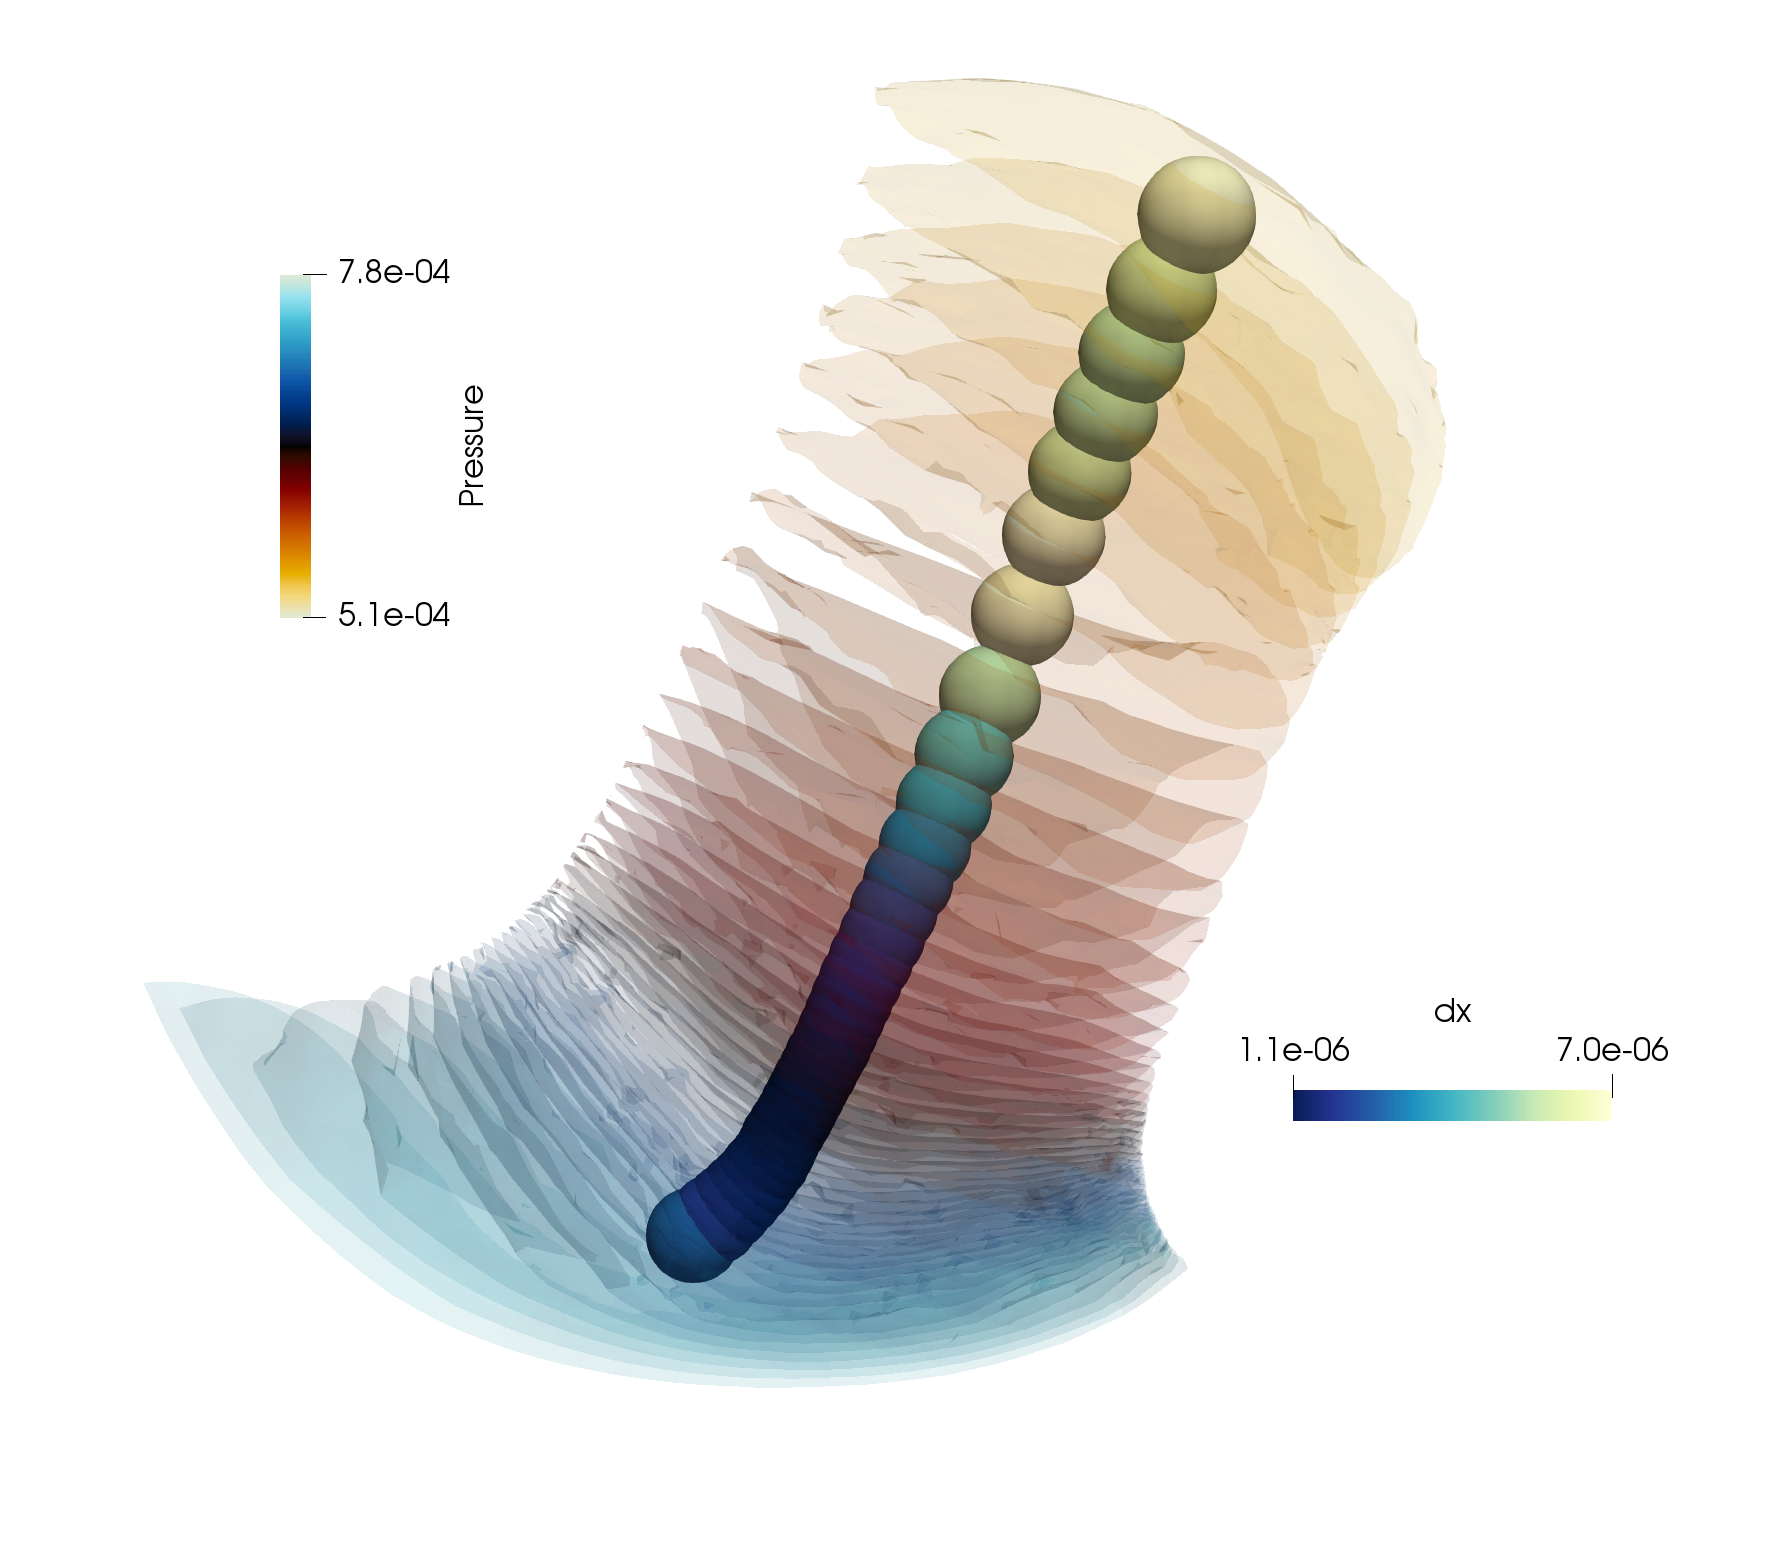
\includegraphics[height=5cm]{figures/example_pore.png}~~~~
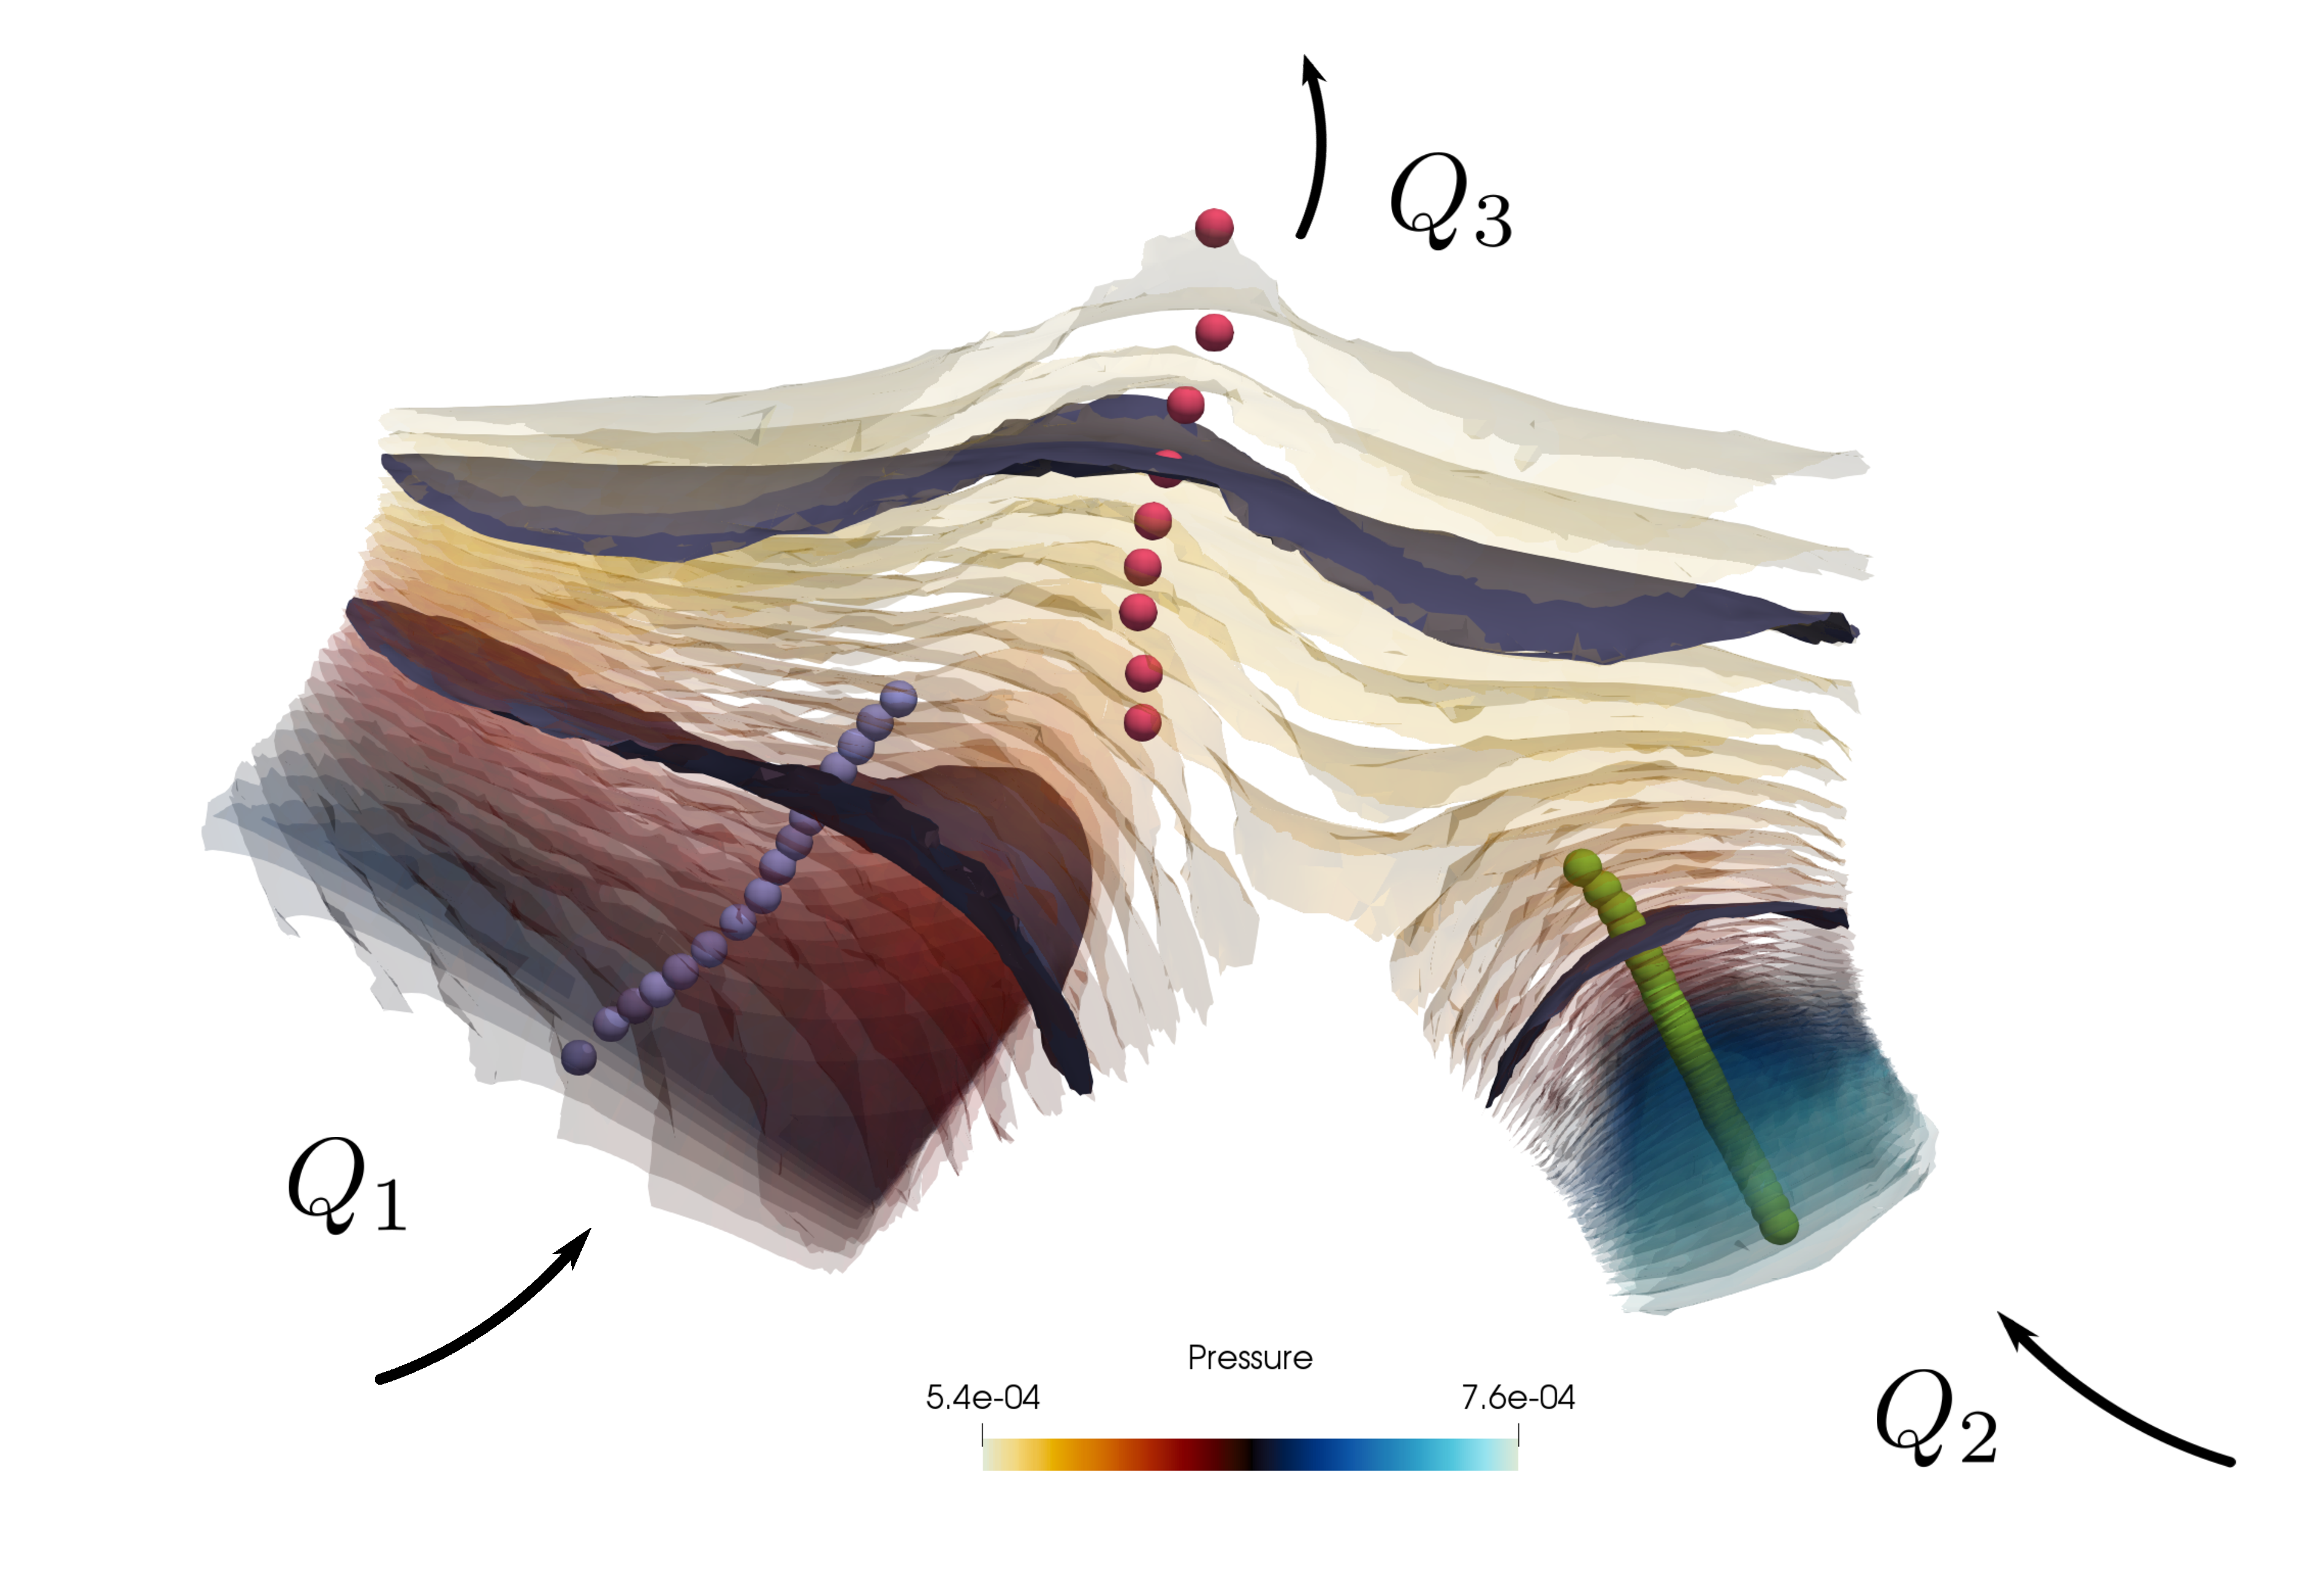
\includegraphics[height=5cm]{figures/merging_pores.eps}
\caption{Left: A visualization of a collection of consecutive iso-pressure surfaces comprising one pore, including the average coordinates of the iso-pressure surfaces indicated by the spheres. The color code of the spheres is given by the distance between the average coordinates between two consecutive iso-pressure surfaces. Right: A visualization of a junction of three pores for which the total flux is conserved $Q_1+Q_2 = Q_3$. This visualization is based on a subset of the DNS results of porous media \#2}
\label{fig:isop_surfaces}
\end{figure}


Here we introduce the notion of disconnected iso-pressure surface $\mathcal{S}_i(p)$ for a given pressure value $p$. Note that this consideration works for any fluid tube bounded by iso-pressure surfaces and iso-pressure surface of velocity magnitude at which velocity is (approximately) zero. Considering completely saturated conditions the boundary terms of Eq.~(\ref{eq:stokes_dissipation}) will drop when multiple pores are added (meaning $\mathbf{n}\rightarrow -\mathbf{n}$). Therefore Eq.~(\ref{eq:stokes_dissipation}) intrinsically only evaluates
\begin{equation}
Q \Delta p=\mu\int (\nabla \mathbf{u})^2 dV.\label{eq:pore_based_energy_dissipation}
\end{equation}

We apply a decomposition of the velocity vector  $\mathbf{u} = u_p \mathbf{\hat{p}} + u_r \mathbf{\hat{r}}$ with $\mathbf{\hat{p}} =\mathbf{ \nabla}p/|\mathbf{ \nabla}p|$. For Hagen-Poiseuille (HP) flow $\mathbf{u}$ is parallel to the pressure gradient, for which in simple geometries exact solutions can be derived. In the following we will assume that the most important contributions to the viscous dissipation tensor $\nabla_i u_j$ is given by $\nabla_i u_p$ i.e. $\mathbf{\nabla}_i u_r \ll \mathbf{\nabla}_i u_p $. This assumption has been verified in the SI for the porous media that we have used below. This assumption leads to 

\begin{equation}
\left|\nabla_i u_j\right|^2 \approx  \left|\nabla_r u_p\right|^2 + \left|\nabla_p u_p\right|^2 .\label{eq:reduced_dissipation_tensor}
\end{equation}

Here the first term is expected to be more important for gradually varying pore geometries since gradients in the velocity in the longitudinal direction are usually much lower than in transverse direction. Equations (\ref{eq:stokes_local})-(\ref{eq:reduced_dissipation_tensor}) are valid for arbitrary volumes $V$. When we consider viscous dissipation of an \textit{infinitesimal} enclosed volume $dV$ defined by $\mathcal{S}_i,\mathcal{S}_{i+1}$ and their respective areas $A_i, A_{i+1}$, separated by average distance $dx$ we can estimate the first term of Eq.(\ref{eq:reduced_dissipation_tensor}) analogous as shown in \cite{mortensen_reexamination_2005} with
\begin{equation}
	\left|\nabla_r u_p\right|^2 =8\pi\mu \left(\alpha_0+\alpha_1\,\mathcal{C}\right)\frac{ Q^2}{A^3}~~~ \rm{with}~~~ ,\label{eq:tau_1}
\end{equation}
with circularity parameter $\mathcal{C} = \mathcal{L}^2/4\pi A(p)$ with perimeter $\mathcal{L} = \int_{\partial \mathcal{S}_i}dl$. The circularity parameter is related to the compactness factor $C = \mathcal{C}/4\pi$ in \cite{mortensen_reexamination_2005}. The coefficients $\alpha_1$ and $\alpha_2$ can be calculated (in first order of compactness) analytically and numerically for simple shapes of the iso-pressure surfaces, such as squares, triangles, or a perturbation of a sphere by spherical harmonics \citeA{mortensen_reexamination_2005}. For heterogeneous media the class of shapes are generally unknown and not symmetric. 
For the second, longitudinal term, we can assume that the total flux $Q$ remains constant for $p\rightarrow p+dp$, and the change of velocity is caused by a change in cross-sectional area $A_i$, or in other words, the channelization of the pore 
\begin{equation}
	\left|\nabla_p u_p\right|^2 = \alpha_2  \frac{Q^2}{A^4}\left|\frac{\partial A}{\partial x }\right|^2,\label{eq:tau_2}
\end{equation}
with unknown $\alpha_2$. For the case where the infinitesimal pressure difference $dp$, no topological changes (no junctions) of the iso-pressure surfaces take place, we can write $dV = A dx$ with $dx$ the average distance between two isolated isopressure surfaces. We  combine the two expressions Eq.(\ref{eq:tau_1}) and Eq.(\ref{eq:tau_2}) with Eq.(\ref{eq:pore_based_energy_dissipation}) into

\begin{equation}
	\frac{dp}{dx} = 8\pi \mu \frac{Q(p)}{A(p)^2} f\left(\alpha_i,\mathcal{S}(p) \right) = 8 \pi \mu\frac{Q}{A^2}\left(\alpha_0+\alpha_1\mathcal{C} + \alpha_2 \frac{1}{A}\left|\frac{\partial A}{\partial x}\right|^2\right)\,\label{eq:infi_dp}
\end{equation}
This expression is consistent with the Hagen-Poiseuille equation for pipe geometries $f(\alpha_i)\rightarrow 1$, for which the local infinitesimal pressure gradient is given by 

\begin{equation}
	\frac{\partial p}{\partial x} = 8 \pi \mu\frac{Q}{A^2}, \label{eq:HP}
\end{equation}
hereafter referred to as the HP-model. As long as there are no junctions Eq.(\ref{eq:infi_dp}) can be integrated. This restriction is therefore used to define a single pore. The total pressure gradient along a pore is then given by

\begin{equation}
	\frac{\Delta p}{L_{\rm{eff}}} =  Q \frac{1}{L_{\rm{eff}}}\int^{L_{\rm{eff}}}_{0}\frac{1}{A^2}f\left(\alpha_i,\mathcal{S}(p)\right)\,dx
\end{equation}

with 
\begin{equation}
	L_{\rm{eff}} = \int^{L_{\rm{eff}}}_{0} dx,
\end{equation}
and $\Delta p$ the pressure difference between the inlet and the outlet of a pore. From this we find an expression for a model for the total hydraulic resistance 

\begin{equation}
	\mathcal{R}_m = \int^{L_{\rm{eff}}}_{0}\frac{1}{A^2}f\left(\alpha_i,\mathcal{S}(p)\right)\,dx\label{eq:R_model}
\end{equation}

When the geometry of a media is given by a long pipe, the hydraulic resistance is given by the Hagen-Poiseuille law $R_m = R_{\rm{HP}}$, meaning that $f(\alpha_i)\rightarrow 1$ and will therefore only depend on the cross-section area  $A(p)$.



\section{Methods}
\begin{figure}[t!]
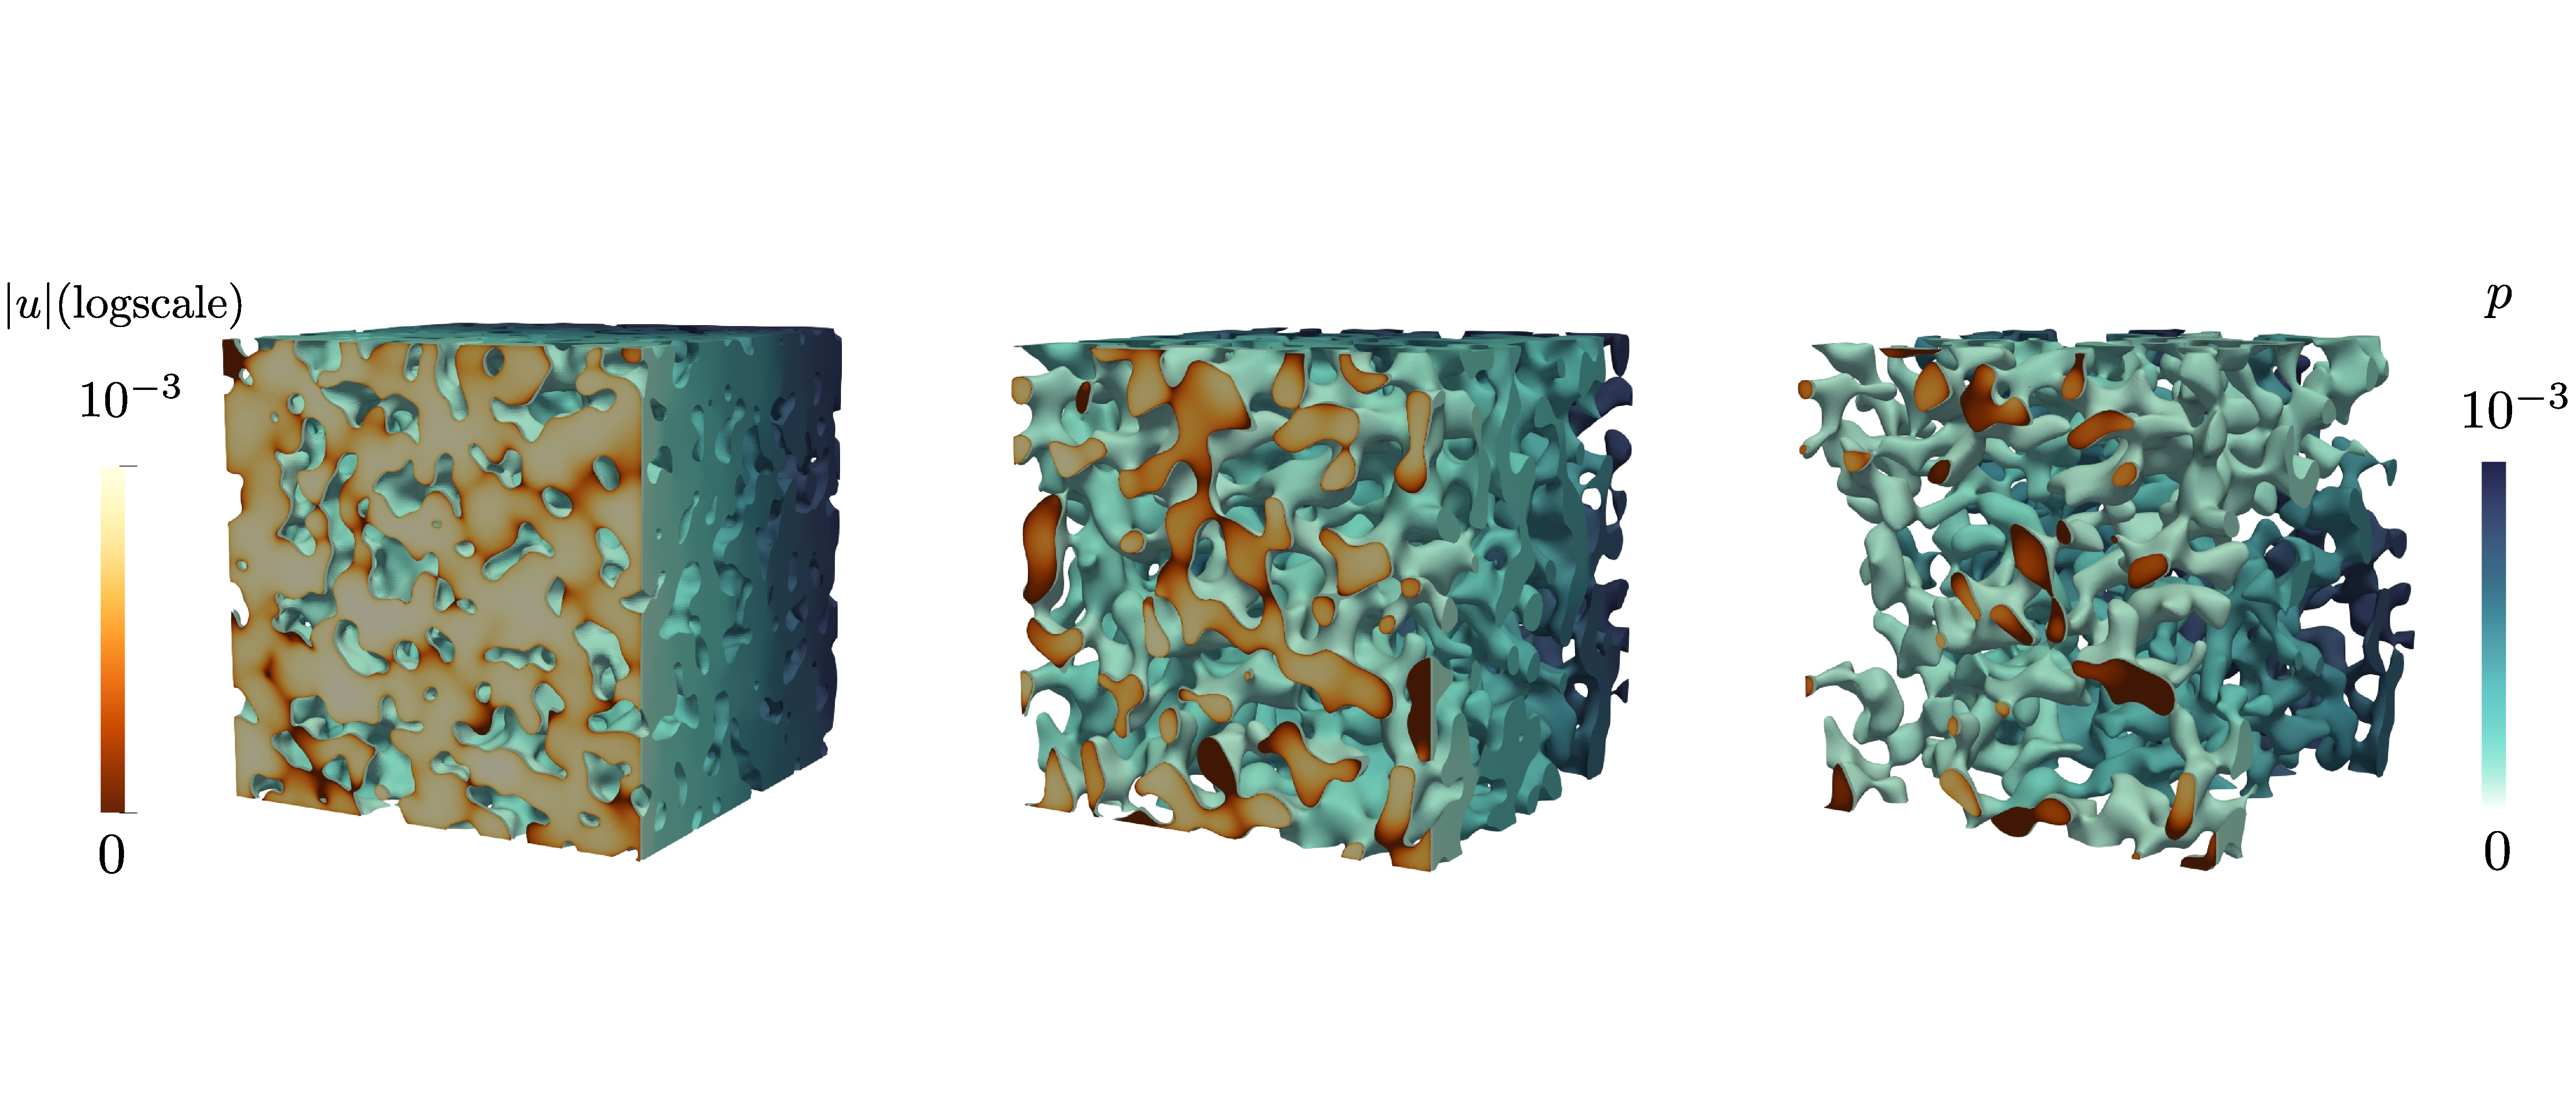
\includegraphics[width=1.0\linewidth]{figures/DNS_overview.eps}
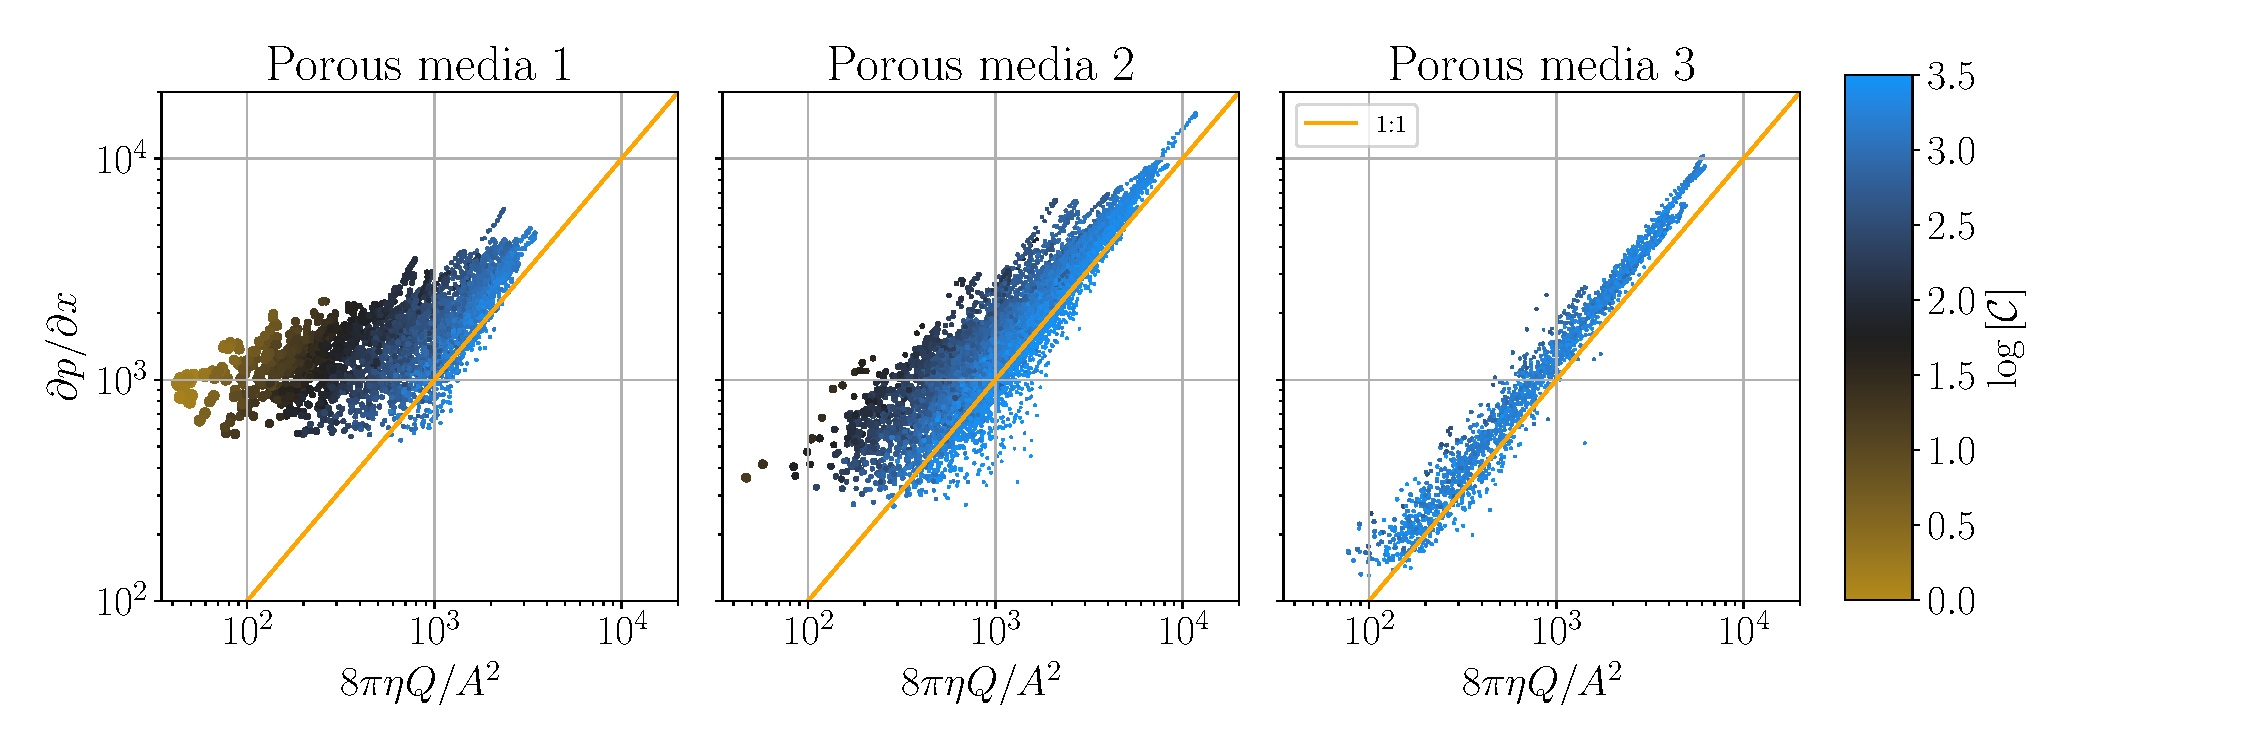
\includegraphics[width=1.2\linewidth]{figures/infi_dpdx_3.pdf}
\caption{Top: A visualization of the velocity field $|u|$ and pressure field $p$ in the pore space of the three porous media used in this study. Bottom: Measurements of local pressure drop versus the Hagen-Poiseuille model given by Eq.(\ref{eq:HP}) hydraulic resistance for three different porous media, the color is given by averaged circularity $\mathcal{C}(p)_i$ and the marker size is scaled with the averaged area $A(p)_i$ of two consecutive iso-pressure surfaces $\mathcal{S}(p)_i,\mathcal{S}(p+\delta p)_j$. }
\label{fig:DNS}
\end{figure}


To generate heterogeneous porous media, that will form the basis for the direct numerical simulations, we have used Gaussian Random Fields (GRF) to generate 3 porous media \cite{teubner_level_1991,hyman_heterogeneities_2012,siena_relationship_2014}. A threshold of the field function of the GRF is used to define the porous media-fluid interface $\Gamma$ with porosities $0.68, 0.34$ and $0.17$ respectively. In the SI we have listed a few geometrical parameters such as average pore size, and surface roughness. These porous media are used as input for direct numerical simulations (OpenFOAM v. 4.1, \citeA{weller_tensorial_1998}), that solves the steady state Navier-Stokes equations in the pore space. The boundary conditions are defined at the inlet $p_1$ and outlet $p_2$ and a no-slip for the porous media-fluid interface. A visualization of the three porous media is shown in Fig.~\ref{fig:DNS}. Then a chain of visualization toolkit (VTK) based image analysis techniques \cite{schroeder_visualization_2006,hernderson_paraview_2007} are employed to extract iso-pressure surfaces $\mathcal{S}(p)$ and enumerate the disconnected areas identifying as an iso-pressure slice $\mathcal{S}_i(p)$, part of a pore and measure its surface area $A_i(p)$, circularity $\mathcal{C}_i(p)$, average location $\mathbf{x}_i(p)$ and average flux $Q_i(p)$. For each $\mathcal{S}_i(p)$ its closest neighbor $\mathcal{S}_j(p+\delta p)$. This neighbor $j$ is found by employing the distance function $f_d(\mathbf{x},\mathcal{S})$, between point $\mathbf{x}$ and surface $\mathcal{S}$ defined by 

\begin{equation}
	f_d\left(\mathbf{x},\mathcal{S}\right) = \min \{\Vert\mathbf{x}-\mathbf{y}\Vert \} ~|~ \mathbf{y}\in \mathcal{S}.
\end{equation}
The index $j$ of corresponding to the minimum value of the averaged distance matrix 
\begin{equation}
	d_{i,k} = \frac{1}{A_i(p)}\int_{\mathcal{S}_i(p)} f_d(\mathbf{x}_i,\mathcal{S}_k(p+\delta p)) \,dS_i, ~\textrm{with}~ A_i(p) = \int_{\mathcal{S}_i(p)}\,dS_i.
\end{equation}
By forward integration of the first iso-pressure patches $\mathcal{S}_i(p_0)$ we identify all patches belonging to the same pore $\mathcal{P}_l(\Delta p) = \{\mathcal{S}_k(p_i)\}$. Since the averaged distance $d_{i,k}$ between two iso-pressure surfaces is very sensitive to topological changes, a maximal distance $dx_{\rm{max}}$ between two consecutive coordinates is used to define the end and the beginning of a pore. A visualization of such a topology change, or splitting and merging of pores is shown in Fig.\ref{fig:isop_surfaces} (Right).

The main challenge with the data format of the OpenFoam simulations is that it is unstructured, and the meshing is refined towards the boundary of the porous media $\Gamma$. Although this ensures that the geometry is accurately described and that the simulation convergences, it also causes problems by extracting $\mathcal{S}(p)$ by using VTK contour filter. Since it is based on a threshold on $p$ it breaks up the mesh close to $\Gamma$ into many disconnected small area patches. To remove these small patches a threshold of a relatively low value for $\left|u\right|< \epsilon$ is chosen. This results in much smoother, but slightly smaller iso-pressure surfaces. The loss of area can be estimated and corrected for each pore individually by $A(p)\rightarrow A(p) + \left.\mathcal{L}\epsilon/\overline{\nabla u}\right|_{\partial \mathcal{S}}$. If this correction is omitted it will result in a significant proportion of values measured pressure gradients below the HP-model, which is physically impossible. Evidently this deviation was mostly observed for relatively small pores. The estimate for $\mathcal{C}$ is subsequently also underestimated if $\epsilon$ is chosen too high. It is however difficult to get a reliable estimate for $\mathcal{C}$ when $\epsilon \rightarrow 0$ because $\partial \mathcal{S}(p)$ becomes irregular. Therefore, we have chosen to estimate $\mathcal{C}$  at finite $\epsilon$, there where it is most robust. $\epsilon$ was chosen to be $2\times10^{-5}$ for the first two porous media and $2\times10^{-6}$ for the last. These values where chosen by visual inspection, not to loose to much detail of the shape of $\mathcal{S}$ and to get rid of most of the noise at the edges. Small area patches that remain are filtered out based on their size. The distance $dx_{\rm{max}}$ is chosen such that upon visual inspection, clearly connected surfaces remain connected, such as can be seen in Fig.\ref{fig:isop_surfaces}(left). A more specific description of the chain of the VTK image analysis techniques is detailed in the SI. 

For each of the three porous media we can plot the local pressure gradient versus the PH model, i.e. Eq.(\ref{eq:infi_dp}) for all consecutive iso-pressure pairs $\mathcal{S}_i(p)$ and $\mathcal{S}_j(p+\delta p)$. To obtain measured values for the resistance of a pore, we divide the total pressure difference $\Delta p$ by the total fluxe $Q$. We fit Eq.(\ref{eq:R_model}), to all pores belonging to one porous media, yielding three sets of $\alpha_i$'s.  


\section{Results}


The result of the DNS for the three porous media is shown in Fig.\ref{fig:DNS}. The Reynolds number is estimated by $Re \sim l_p q/\nu$, with $q = Q/\overline{A}$ and is smaller than $10^{-2}$ for all three media. In Fig.\ref{fig:DNS}, bottom, the results of the infinitesimal pressure gradients versus the HP model (Eq.(\ref{eq:HP})) are shown. We observe that the HP model underestimates the pressure gradient up to two orders of magnitude for the first porous media, to a relative good estimate for the third. We observe that the smaller the pores are, the smaller is $\mathcal{C}$, indicating that smaller iso-pressure surfaces are compacter than the larger more complexed shaped iso-pressure surfaces. In Fig.\ref{fig:local_and_integrated} (top left) we have plotted the joined datasets of the three porous media. We observe that after joining the datasets there is no visual distinction between the three porous media, i.e. their data overlap and behave uniformly with respect to $\mathcal{C}$ and $A$.
 
For each porous media Eq.(\ref{eq:infi_dp}) has been fitted by minimizing the least-squared independently to obtain estimates for $\alpha_i$. The values for $\alpha_0 =[0.26,0.40,0.98]$, $\alpha_1 = [0.72,0.69,0.32]$, and $\alpha_2 = [4.7\times 10^{-3},1.3 \times 10^{-3},0.22]$. The relative contribution of the first and second term of $f(\alpha_i)$ are given by $[14\%,29\%,69\%]$, $[86\%,71\%,30\%]$ for $\alpha_0$ and $\alpha_1$. The relevance of the last term can be deduced to be irrelevant ($\leq1\%$). The obtained modelled local pressure gradient by Eq.(\ref{eq:pressuredrop}) using the newly obtained $f(\alpha_i)$ is shown in Fig.\ref{fig:local_and_integrated}(top right). We observe that for the first two porous media the circularity is the most relevant parameter ($\alpha_1$). For the last porous media the HP contribution ($\alpha_0$) is the most relevant. The relative contributions of the HP-model, i.e. ($\alpha_0$ to $\alpha_1\mathcal{C}$) is increasing with decreasing porosity. When the porosity is doubled the relative contribution of $\alpha_0$ is roughly divided by two. For the third porous media we observe that the relative contribution of circularity is the smallest. This is to be expected since the pores are characterized with circularity close to 1 (see SI for a quantitative comparison in Fig.\ldots). The Pearson correlation coefficients for these models are $0.93, 0.98, 0.99$ respectively. Because our data spans more orders of magnitude and the HP model entails a high degree of heteroscedatisticy \citeA{white_heteroskedasticity-consistent_1980}, the Pearson correlation coefficient is not very reliable measure for the goodness of fit \citeA{wilcox_comparing_2009}. The ratio of root-mean-squared-relative error (RMSRE) is not effected by the latter. The ratio of the RMSRE of the circularity-based model and the HP model is given by $0.33, 0.67$ and $0.87$, showing that the most improvement is found for the first porous media, which is in agreement with Fig.\ref{fig:DNS} (bottom).



\begin{figure}
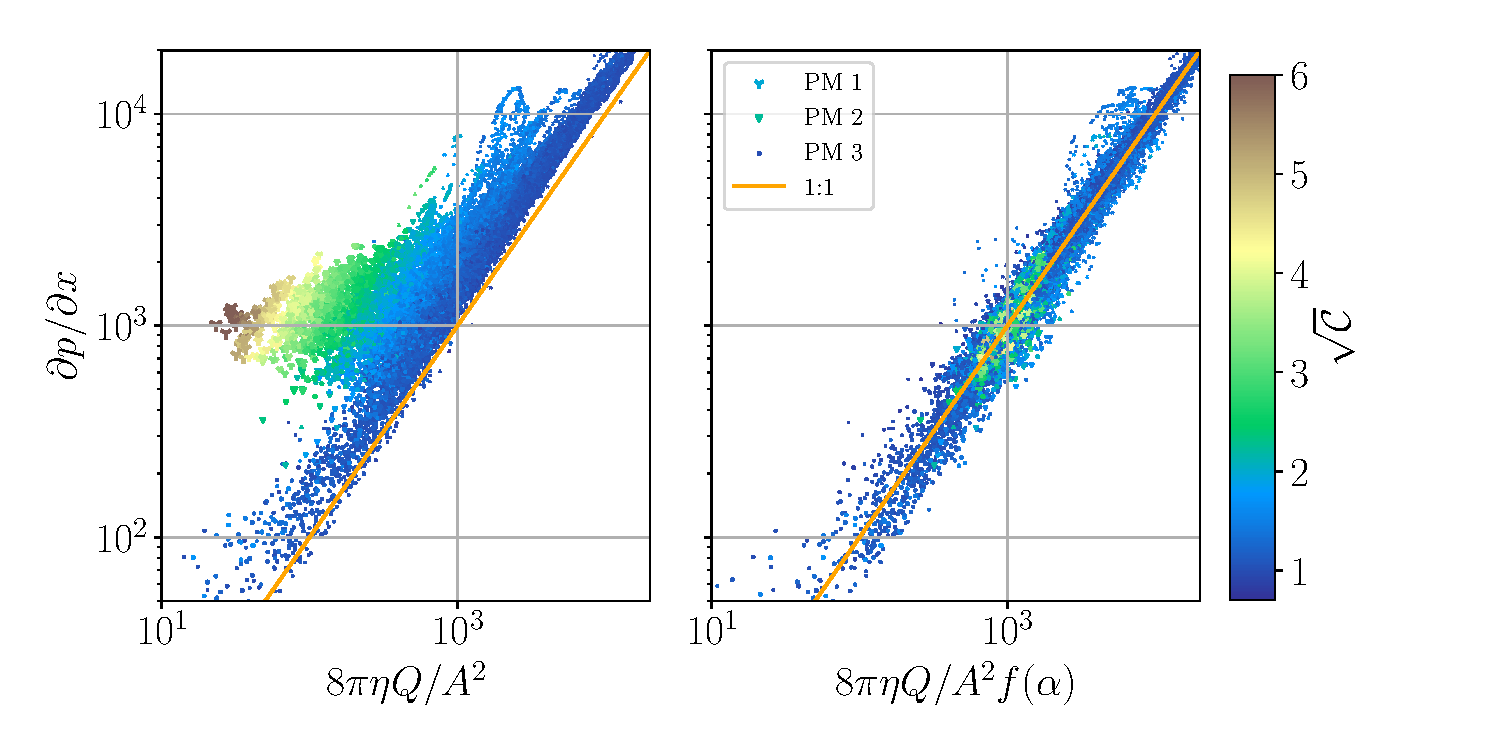
\includegraphics[height=8cm]{figures/infi_dpdx_combined.pdf}
\includegraphics[height=8cm]{figures/integral_dpQ_combined.pdf}
\caption{Top left: Measured infinitesimal pressure gradient versus the infinitesimal pressure drop of a Hagen-Poiseuille model, i.e. $f(\alpha)\rightarrow 1$, for all three porous media combined. The relative cross-sectional area $A_i(p)$ is given by the markersize. Top right: Measured versus Modeled infinitesimal pressure gradient with $f(\alpha)$ fitted to Eq.(\ref{eq:R_model}) for each porous media separately. Bottom: The marker size is scaled by averaged area of the pore. Left: Integrated pressure drop vs $\mathcal{R}_{HP}$ times the total Flux $Q$ Right: Integrated pressure drop divided by the total Flux $Q$ vs $\mathcal{R}_m$ (Eq.(\ref{eq:R_model}). }
\label{fig:local_and_integrated}
\end{figure}


Retrieving measured and modelled (HP-model and the new model) data for the resistance of a pore, it only requires integration of Eq.(\ref{eq:infi_dp}) along a pore, i.e. evaluating $\Delta p/Q$ and Eq.(\ref{eq:R_model}). The results for the HP model ($f(\alpha_i)\rightarrow1$) are shown in Fig.(\ref{fig:local_and_integrated})(bottom left). The results for our model Eq.(\ref{eq:R_model}) are shown in Fig.(\ref{fig:local_and_integrated})(bottom left).

Since we obtain a range of complex shapes for $\mathcal{S}$ the obtained values for $\alpha_i$ are expected to be an average. We have tested a uniform approach by setting $\alpha_2 = 0$ and constraining $\alpha_0$ and $\alpha_1$ (consistent with $f(\alpha)\rightarrow 1$ if $\mathcal{C} \rightarrow 1$) by 

\begin{equation}
	\mathcal{R}_m = \int^{L_{\rm{eff}}}_{0}\frac{1}{A^2}\left(1-\alpha\left[1-\mathcal{C}\right] \right)\,dx\label{eq:R_model_uniform}.
\end{equation}

We fitted this model by minimizing the RMSRE, to find $\alpha =[0.62, 0.62, 0.71]$. for the porous media respectively. The fit was performed after integration, meaning that each pore contributes with one data point. The RMSRE is given by $[0.21,0.21,0.17]$, which significantly improves on the RMSRE of the HP model ($\alpha = 1$) given by $[0.62,0.42,0.25]$. A sensitivity plot of $\rm{RMSRE}_m/\rm{RMSRE}_{HP}$ on $\alpha$ can be found in the SI including measures of statistics of all the models used in this paper.



\section{Discussions}

One of the most important findings is that the prediction of the resistance of a pore by the HP-model is highly underestimated with an average RMSE of \ldots. This is most pronounced when the pores have a complex geometry, which are usually correlated with large pore areas, see Fig.\ref{fig:local_and_integrated}. An average underestimation of the resistances leads to an average overestimation of the mean fluxes in a network model. This will affect transport predictions e.g. breakthrough times will be underestimated \cite{dentz_mechanisms_2018}. Network models such as \cite{alim_local_2017}, often base their local resistances on the smallest distances to the porous media boundary. In general this will underestimate the cross-sections and therefore obtain higher resistances for the HP-based model, also reducing the error with respect to our HP model. Since anomalous diffusion has been correlated with the degree of heterogeneity of the porous media, it is important that low flux regions are included. The inaccurate representation of the low velocity regions by larger cross-sectional areas will therefore contribute to poor estimates of anomalous long residence times. This will lead to non-Fickian scaling behaviour of the dispersion of flow tracers \cite{dentz_mechanisms_2018,dentz_delay_2006}.

Extrapolating our results to more homogeneous media such as packed-beads, sandstone and ordered media such as used by \cite{alim_local_2017}, might be challenging. In orderd media we might expect difficulties in retrieving statistics on the iso-pressure surfaces. For high porosities these might be too connected, and sometimes even consist of a single iso-pressure surface, occasionally without holes. We therefore expect our results to be significant when significant disorder of the grains is in place. One possible roadmap for separation of highly connected iso-pressure surfaces into smaller pores is by using a Morse-Smale-Complex segmentation e.g. from the Topology ToolKit \cite{tierny_topology_2018}. We have implemented this method, for porous media 1, with similar results, which are visualized and shortly described in the SI. 

The range of local resistances in Fig.\ref{fig:local_and_integrated}(bottom) show that low resistances are correlated with high values for $\mathcal{C}$, and are poorly estimated by HP. These pores are crucial for predicting preferential flow paths since they depend on the paths of least resistances throughout a network. For this purpose we have computed the RMSRE weighted by the mean flux. We found a reduction from $67\%, 30\%, 6\%$ to $2\%, 2\%,5\%$ for three heterogeneous respectively, which shows a remarkable improvement of high flux pores.  

One of the key observations of our work is the possibility of introducing a local geometric factor that provides for the ratio of pressure difference and mass flux in a given channel. The factor depends on the considered channel and not the rest of the complicated shape of the medium boundary. The non-triviality of this observation is made transparent by employing the boundary integral representation which is equivalent to the Stokes equations obeyed by the flow. The representation gives the flow as an integral over the medium surface where the points of the surface appear as sources that produce the flow as superposition. The ``charge" of such sources is proportional to the stress tensor at the boundary and the flow that each charge induces in space is given by an appropriate Green's function, see e.g. \cite{pozrikidis_boundary_1992}. Our result demonstrates that contributions other than those from the boundary of the considered channel can be neglected in the superposition. The mechanism by which this occurs, consists of both screening effect and destructive interference between different channels. This deserves further studies which are beyond our scope here. We have used circularity, as a single measure for the shape of $\mathcal{S}(p)_i$, but to improve on this result it might be necessary to include other shape parameters such as curvatures measures of $\mathcal{S}(p)_i$, which may lead to non-linear behavior in a circuit model. 

Although the proposed definition of individual pores deals naturally with junctions, a straight forward pore-network implementation is still missing. Given that the distributions of the resistances show similarity with a log-normal distribution, a statistical pathway for a statistical network based on these distributions seem feasible.  



\section{Conclusions}
We have proposed a new iso-pressure surface based definition for individual pores in heterogeneous porous media with the aim of measuring and modeling the local hydraulic resistance which can potentially be used in a pore-network model. This new definition uses the constant flux as constraint on the length of the pore. The definition of the pores allows us to estimate the local hydraulic resistance in terms of the viscous dissipation tensor. This can be modeled by the circularity of the iso-pressure surfaces which significantly improves the Hagen-Poiseuille model for high porosity heterogeneous media. 





\acknowledgments{Q. Krol acknowledges dr. H.L\"owe for valuable discussions and  M. Holzner acknowledges grant ... }



\bibliography{library.bib}



\end{document}



